\documentclass[9pt,aspectratio=169]{beamer}

\usepackage{nicefrac}
\usepackage{ragged2e}
\usepackage{tabularray}
\usepackage{luamplib}
\everymplib{input mpcolornames; input repere; beginfig(1);}
\everyendmplib{endfig;}

\usetheme{graham}

\title{Rate problems}
\subtitle[Graham Middle School]{Graham Middle School Math Olympiad Team}

\begin{document}
\maketitle

\begin{frame}{Rate and units}
  \begin{columns}[T]
    \begin{column}{0.5\textwidth}
      \begin{definition}
        A \textbf{rate} is a measure of how a quantity is changed over time.
      \end{definition}
      Rates, though, can be used to measure many different quantities. Suppose you can finish $10$ MOEMS problems in $30$ minutes.  Then the rate at which you do the math problems is $\dfrac{10\text{ problems}}{30\text{ minutes}}$ or $\nicefrac{1}{3}$ of a problem per minute.
      \begin{problem}
        How many MOEMS problems can you finish in an hour if you do $\nicefrac{1}{3}$ problem per minute?
      \end{problem}\vspace*{-0.7em}
      \[ \dfrac{1\text{ problem}}{3\text{ min}} \times 60 \dfrac{\text{min}}{\text{hour}} = 20 \dfrac{\text{problems}}{\text{hour}}.\]
      When converting between units, track and cancel the units like numbers. In this problem, the minutes units in the numerator and denominator cancel, leaving us with problems/hour. 
    \end{column}
    \begin{column}{0.5\textwidth}
      When dealing with rate problems, it’s important to pay attention to the units.
      
      It is helpful to know some unit conversions.\smallskip

      \emph{Time}

      $1$ minute $= 60$ seconds;

      $1$ hour $= 60$ minutes $= 3{,}600$ seconds;

      \mbox{$1$ day $= 24$ hours $= 1{,}440$ minutes $= 86{,}400$ secs.}\smallskip

      \emph{Distance} (metric)

      $1$ cm (\emph{centi}meter) $= 1$ mm (\emph{milli}meter); 

      $1$ m (meter) $= 100$ cm $= 1000$ mm;

      $1$ km (\emph{kilo}meter) $= 1000$ m.\smallskip

      \emph{Distance} (imperial)

      $1$ in (inch) $= 25{.}4$ mm;

      $1$ ft (foot) $= 12$ in $= 30{.}48$ cm;

      $1$ yd (yard) $= 3$ ft $= 91{.}44$ cm $\approx 1$ m;

      $1$ mi (mile) $= 5{,}280$ ft $= 1609{.}344$ m $\approx 1{.}5$ km.\smallskip

      \emph{Speed}

      $1$ m/s (meter per second) $= 3{.}6$ km/hr;

      $1$ km/hr $\approx 0{.}62$ mps (miles per hour).
    \end{column}
  \end{columns}
\end{frame}

\begin{frame}{Distance = speed × time}
  \begin{columns}[T]
    \begin{column}{0.5\textwidth}
      The rate you are probably most familiar with is speed. The speed measures what distance is traveled in a given unit of time.  In middle school problems, speed is usually a constant.
      \begin{problem}
        Maya is running a $5$ km race.  If she finishes the race in $20$ minutes, what was her average speed in km/hr?
      \end{problem}
      \begin{wrapfigure}{r}{0.3\textwidth}
        \vspace*{-1.3em}\hspace*{-2em}
        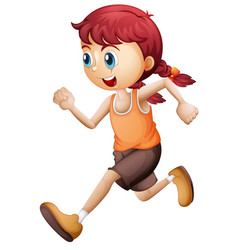
\includegraphics[width=0.4\textwidth]{09 - Rate/run.png}
      \end{wrapfigure}
      She finishes in $20$ min which is $\nicefrac{1}{3}$ of an hour.  Since $\text{distance} = \text{avg. speed} \times \text{time}$, $5\text{ km} = \text{avg. speed} \times \nicefrac{1}{3}\text{ hour}$. So her average speed was $15$ km/hr.
      \vspace*{2\baselineskip}
      \begin{definition}
        {\centering 
        $d = s \times t$,\par
        }
        
        where $d =$ distance, $s =$ rate, which is the average speed, and $t$ is time.
      \end{definition}
    \end{column}
    \begin{column}{0.5\textwidth}
      \begin{problem}
        If it takes $8$ minutes for photons to travel the $150$ million km from the Sun to Earth. What is $c$, the speed of light in m/sec?
      \end{problem}
      Since $d = c \times t$, the speed of light. First, we need to convert everything to needed units. $150$ million km is $150$ billion meters, e.g. $1{.}5 \times 10^{11}$ meters. $8$ minutes is $8 \times 60 = 480$ seconds
      \[ c = \frac{1{.}5 \times 10^{11}\text{ m}}{480\text{ sec}} \approx 3 \times 10^8\text{ m/s}.\]\vspace*{-0.7em}
      \begin{example}
        Tip 1:  Always check the units in rate problems to be certain you are answering the question that is being asked.  There is seldom partial credit on these contests, and giving the speed in km/s when the question asks for m/s is a painful way to miss a~question.

        Tip 2: If a problem uses different units (like minutes and seconds), converting all values to the same units will prevent many errors. 

      \end{example}
    \end{column}
  \end{columns}
\end{frame}

\begin{frame}{Multispeed trips}
  \begin{columns}[T]
    \begin{column}{0.5\textwidth}
      What if the speed on a trip is not constant?  In that case, the total distance is still the average speed times the total time, but we divide the trip up into the segments at different speeds.
      \begin{definition}
        {\centering
        $d = s_1 \times t_1 + s_2 \times t_2 + \ldots$,\par} 
        where $t_i$ represents the time spent at speed $s_i$.
      \end{definition}
      \begin{problem}
        Sam lives at the top of a steep hill.  When he bikes downhill, it takes him $2$ minutes to reach the base of the hill.  If it takes him $10$ minutes to bike up the hill, what is his average speed for the roundtrip if the hill is $1$ mile long?
      \end{problem}\vspace*{-1em}
      \[\text{total distance} = \text{average speed} \times \text{time}. \]
      The total distance is $2$ miles.  The total time is $12$ minutes.  The average speed is 
      \[ \frac{2\text{ miles}}{12\text{ minutes}} = \frac{1}{6}\text{ mi/min or $10$ mph}. \]
    \end{column}
    \begin{column}{0.5\textwidth}
      Note that the speed going downhill is 
      \[ \frac{1 \text{ mi}}{2 \text{ min}} = \frac{1}{2}\text{ mi/min} = 30\text{ mph}, \] 
      and the speed going uphill is 
      \[ \frac{1 \text{ mi}}{10 \text{ min}} = \frac{1}{10}\text{ mi/min} = 6\text{ mph}. \]
      \begin{wrapfigure}[9]{r}{0.4\textwidth}
        \vspace*{-1.8em}\hspace*{-1.5em}
        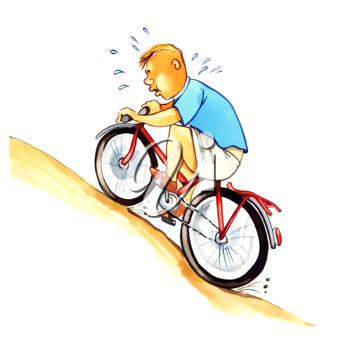
\includegraphics[width=0.5\textwidth]{09 - Rate/bike.png}
      \end{wrapfigure}
      The average speed is not the average of $30$ mph and $6$ mph which would be $18$ mph.  That is because Sam spends $5$ times a long biking uphill as he does biking downhill.  If you weight the average by the ratios of the times spent at the two speeds, you will calculate the
      \[ \text{average speed} = \frac{5}{6} \times 6 + \frac{1}{6} \times 30 = 10\text{ mph}.\]
    \end{column}
  \end{columns}
\end{frame}

\begin{frame}{Wind and current}
  \begin{columns}[T]
    \begin{column}{0.5\textwidth}
      Sometimes there are environmental factors that affect the speed of a boat or plane.  Wind and water currents are the two most common factors.  When a boat or swimmer is going downstream, the speed of the current is added to their normal speed.  When they are going upstream, the speed of the current is subtracted from their normal speed.

      {\centering
      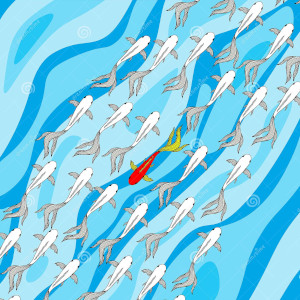
\includegraphics[width=0.65\textwidth]{09 - Rate/fish.jpg}\par}
    \end{column}
    \begin{column}{0.5\textwidth}
      Wind speed is treated in a similar manner.  When the wind is at your back, you are said to have a~tailwind, and the wind speed is added to your normal air speed.  Conversely, when you are going into a headwind, the wind is blowing against you, and the wind speed is subtracted from your normal air speed.
      \begin{problem}
        Swimming out to the buoy, Ann is going against the current, and it takes her $30$ minutes.  Her return swim, with the current at her back, takes $20$ minutes.  If the buoy is $1$ mile from her starting point, and her speed would be constant without the current, what is the speed of the current?
      \end{problem}
      Let $x$ be the speed of the current, and y be Ann’s speed without the current.  We get a system of two equations: $30(x - y) = 1$ and $20(x+y) = 1$.  Solving them we find Ann swims at a speed of $2{.}5$ mph without current, and the current speed is $0{.}5$~mph.
    \end{column}
  \end{columns}
\end{frame}

\begin{frame}{Circular motion}
  \begin{columns}[T]
    \begin{column}{0.5\textwidth}
      \justifying
      An important group of rate problems involves motion in a circle.  The speed of the motion is often given in terms of \emph{revolutions per minute} (rpm).  To convert this to a rate in terms of distance, we must multiply rpm by the circumference to get distance per minute.  This is simply because for each revolution, we travel a~distance equal to the circumference.
      \begin{problem}
        A hamster is running on its exercise wheel.  If the wheel has a radius of $10$ cm, how fast is the hamster running if the wheel is spinning at a rate of $80$ rpm?
      \end{problem}
      If the hamster appears to be stationary while the wheel spins, it means its speed is equal to the speed of the wheel (just like a treadmill).  The circumference of the wheel is $2\pi r = 20\pi$ cm. 
      \[ 80\text{ rpm} \times 20\pi\text{ cm} = 1600\pi\text{ cm/min}.  \]\vspace*{-1.4\baselineskip}
      \begin{multline*}
        1600\pi\text{ cm/min} = 16\pi\text{ m/min} = {} \\
        {} = 960\pi\text{ m/hr} \approx 3\text{ km/hr}.	                
      \end{multline*}
    \end{column}
    \begin{column}{0.5\textwidth}
      \vspace*{-1em}
      \begin{center}
        \leavevmode
        \begin{mplibcode}
          u=0.65cm;
          path a, b;
          pair ac, bc;
          ac = (0, 0);
          bc = (2u*3.14159, 0);
          a = fullcircle scaled 2u;
          b = a shifted bc; 
          draw a withcolor Gray withpen pencircle scaled 1.25;
          draw b withcolor Gray withpen pencircle scaled 1.25;
          draw (-2u, -u)--(xpart bc + 2u, -u);
          draw ac--(u*dir 220) withcolor Gray;
          draw bc--(bc + u* dir 220) withcolor Gray;
          draw ac--bc withcolor Chartreuse4 withpen pencircle scaled 1.25;
          label.top(btex $2\pi r$ etex, .5[ac,bc]);
          label.lrt(btex $r$ etex, .4u*dir 220);
          label.lrt(btex $r$ etex, bc + .4u*dir 220);
        \end{mplibcode}
      \end{center}
      \begin{example}
        If a wheel is “rolling without slipping” then the distance the center of the wheel moves with each revolution of the wheel is equal to the outer circumference of the wheel.  In the diagram above, the wheel on the left is in the starting position.  After completing one clockwise revolution, the center of the wheel has moved a distance $2\pi r$ to the right.
      \end{example}
      \begin{problem}
        Two balls are rolling along the blacktop at the same speed.  If one ball has twice the diameter of the other, what is the ratio of their rotation rates in rpm?
      \end{problem}
      Since the speed along the blacktop$ = \text{rpm} \times 2\pi r$, the smaller ball’s rpm must be twice as large.
    \end{column}
  \end{columns}
\end{frame}

\begin{frame}{Reduction to unity}
  \begin{columns}[T]
    \begin{column}{0.5\textwidth}
      \begin{problem}
        $40$ walnut trees produce $3600$ lbs of nuts over a $6$ year span.  How many walnut trees produce $2040$ lbs of nuts over an $8$ year span?
      \end{problem}
      It is useful to create this table\smallskip

      \begin{tblr}{width=\textwidth,colsep = 1mm,colspec={X[1.5,c]X[2,c]X[3,c]X[5,p]}}\hline
        years & walnuts & production& description \\\hline
        6 & 40 & 3600 & convert to 1 year \\
        1 & 40 & 600 & convert to 1 tree \\
        1 & 1 & 15 & 1 tree in 1 year
      \end{tblr}
      Now it is easy to calculate an answer during the same thing in reverse order.\smallskip

      \begin{tblr}{width=\textwidth,colsep = 1mm,colspec={X[1.5,c]X[2,c]X[3,c]X[5,p]}}\hline
        years & walnuts & production& description \\\hline
        8 & 1 & 120 & in 8 years \\
        8 & \textbf{17} & 2040 & $\frac{2040}{120} = 17$
      \end{tblr}
    \end{column}
    \begin{column}{0.5\textwidth}
      \begin{problem}
        $60$ deer graze $540$ lbs of grass over a $3$ hours interval. How many deer will graze $300$ lbs of grass over $2$ hours interval?
      \end{problem}

      \begin{tblr}{width=\textwidth,colsep = 1mm,colspec={X[1.5,c]X[1.5,c]X[3,c]X[5,p]}}\hline
        deers & hours & lbs of grass & description \\\hline
        60 & 3 & 540 & convert to 1 deer \\
        1 & 3 & 9 & convert to 1 hour \\
        1 & 1 & 3 & 1 deer in 1 hour \\
        1 & 2 & 6 & in 2 hours \\
        \textbf{50} & 2 & 300 & $\frac{300}{6} = 50$
      \end{tblr}
      
      \centering 
      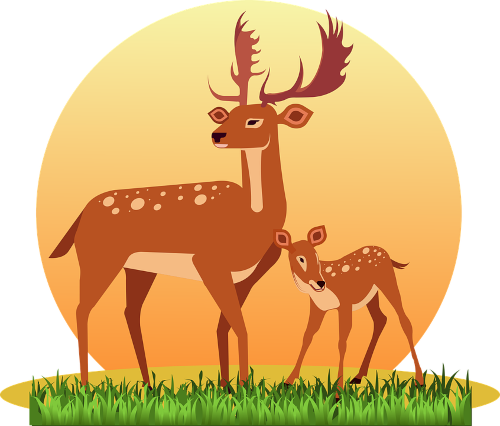
\includegraphics[width=0.45\textwidth]{09 - Rate/deer.png}
    \end{column}
  \end{columns}
\end{frame}

\begin{frame}{Combining work rates}
  \begin{columns}[T]
    \begin{column}{0.5\textwidth}
      In math contest problems, friends working together always seem to work at different rates.  Let $n_i$ equal the number of units the $i$\textsuperscript{th} person produces.  For each person, $n_i = r_i t$.
      \begin{definition}
        The total output is equal to $(r_1 + r_2  + r_3 + \ldots) t$.  In other words, we sum their rates to calculate how much they produce working together for a given time.
      \end{definition}
      \begin{problem}
        Two friends are decorating cupcakes.  If one can decorate a cupcake in $2$ minutes, and the other can decorate a cupcake in $3$ minutes, how long will it take them to decorate $100$ cupcakes?        
      \end{problem}
      Their rates are $\nicefrac{1}{2}$ cupcake/min and $\nicefrac{1}{3}$ cupcake/min.  Their combined rate is $\nicefrac{1}{2} + \nicefrac{1}{3} = \nicefrac{5}{6}$ of a cupcake per minute.  
      \[ 100 = \nicefrac{5}{6}\text{ cupcake/min} \times \text{ time}, \]
      so it will take them $120$ minutes to decorate $100$ cupcakes.
    \end{column}
    \begin{column}{0.5\textwidth}
      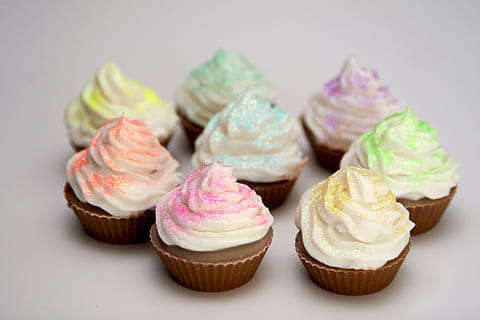
\includegraphics[width=\textwidth]{09 - Rate/cupcakes.jpg}
    \end{column}
  \end{columns}
\end{frame}

\begin{frame}{Exercises}
  \begin{columns}[T]
    \begin{column}{0.5\textwidth}
      \setlength{\leftmargini}{0.2cm}
      \begin{enumerate}
        \item If it takes $5$ minutes for $5$ moles to dig $5$ holes, how many minutes would it take $6$ moles to dig $6$ holes?
        \item Stephan traveled by plane for $4$ hours at an average speed of $600$ mph, then he waited for his luggage for $45$ minutes, and then he drove by car for $75$ minutes at an average speed of $65$ mph. What was his average speed of the travel overall? 
        \item If runner A can run $8$ laps around a course per hour, and runner B averages $8$ minutes to run a lap around the same course, who has run further at the end of an hour, and by how many laps?
        \item Flying $2{,}500$ miles from San Francisco to New York takes $5$ hours, while the flight along the same route from NY to SF takes $6$ hours.  If the plane’s average airspeed would be constant without wind, what was the average jet stream speed in the west-east direction?
        \seti
      \end{enumerate}
    \end{column}
    \begin{column}{0.5\textwidth}
      \setlength{\leftmargini}{-0.1cm}
      \begin{enumerate}
        \conti
        \item Runners A and B run a $50$ meter race, and runner A wins by $10$ m.  If they run a $60$ m race at the same speed, how many meters will runner A win by?
        \item A vinyl record is rotating at a speed of $33$ and $\nicefrac{1}{3}$ revolutions per minute.  How fast is the needle moving over the surface of the record when you are $6$ cm from the center of the album?  How much faster is the needle moving at a distance of $12$ cm from the center?
        \item A bike with $60$ cm diameter wheels is coasting downhill with wheels spinning at $200$ rpm.\\ 
        a) If the wheels are rolling without slipping, what is the speed of the cyclist in cm/min?\\
        b) To the nearest whole number, what is the speed of the cyclist in km/hr.
        \item $2$ pipes are filling a pool with water.  By themselves the pipes would take $3$ and $4$ hours apiece to fill the pool.  How long will it take both pipes together to fill the pool?
      \end{enumerate}
    \end{column}
  \end{columns}
\end{frame}

\begin{frame}{Challenge problem}
  \begin{columns}[T]
    \begin{column}{0.5\textwidth}
      \begin{enumerate}
        \item Consider a road $80$ ft. wide that is $1$ mile ($5{,}280$ ft) long.  Two runners are going to run from the start to the end of the road, but one runner is faster than the other and gives the slower run the following offer:  You can run in straight line down the center of the road (shown in yellow), while I will run along the semi-circular arcs whose diameter is equal to the road width, as shown in black in the diagram.  If the slow runner goes at a speed of $5$ mph, how fast must the other runner run in order to win the race (give your answer in terms of $\pi$)
        
        \begin{center}
          \leavevmode
          \begin{mplibcode}
            u = 0.41cm;
            fill (0, -1u)--(6u, -1u)--(6u, 1u)--(0, 1u)--cycle withcolor AntiqueWhite3;
            draw (0, 0){down}..(u, -1u){right}..(2u, 0){up}..(3u, 1u){right}..(4u, 0){down}..(5u, -1u){right}..(6u, 0){up} withpen pencircle scaled 1.5;
            draw (0, 0)--(6u, 0) withcolor Yellow withpen pencircle scaled 1.5;
            shift = 7.5u;
            fill (shift , -1u)--(shift + 6u, -1u)--(shift + 6u, 1u)--(shift, 1u)--cycle withcolor AntiqueWhite3;
            draw (shift, 0){down}..(shift + u, -1u){right}..(shift + 2u, 0){up}..(shift + 3u, 1u){right}..(shift + 4u, 0){down}..(shift + 5u, -1u){right}..(shift + 6u, 0){up} withpen pencircle scaled 1.5;
            draw (shift, 0)--(shift + 6u, 0) withcolor Yellow withpen pencircle scaled 1.5;
            label.top(btex $\text{start}$ etex, (0, 1u));
            label.top(btex $\text{finish}$ etex, (shift + 6u, 1u));
            pickup pencircle scaled 1.5;
            drawdot (0.25[shift, 6u], 0);
            drawdot (0.5[shift, 6u], 0);
            drawdot (0.75[shift, 6u], 0);
          \end{mplibcode}
        \end{center}
        \seti
      \end{enumerate}
    \end{column}
    \begin{column}{0.5\textwidth}
      \begin{enumerate}
        \conti
        \item The Origami Club at Graham decided to make paper cranes for the school dance.  Working alone, it would take Gabriel, Alyssa, and Valerie $3$, $4$, and $6$ hours respectively to make enough cranes for the dance.  If they work together at the same rate they work individually, how many minutes will it take them to complete the decorations?
        \item Miki has a dozen oranges of the same size and a dozen pears of the same size. Miki uses her juicer to extract $8$ ounces of pear juice from $3$ pears and $8$ ounces of orange juice from $2$ oranges. She makes a pear-orange juice blend from an equal number of pears and oranges. What percent of the blend is pear juice?
        \seti
      \end{enumerate}
    \end{column}
  \end{columns}
\end{frame}

\begin{frame}{Title}
  \begin{columns}[T]
    \begin{column}{0.5\textwidth}
      \begin{enumerate}
        \conti
        \item A current is moving at a speed of $1$ km/h to the right in the diagram.  If you can swim at a~speed of $2$ km/h in still water,\\
        a)  at what angle $\theta$ relative to straight across must you swim in order to reach your friends directly across the river from you? \\
        b)  By swimming at this angle, how much longer will it take you to swim across a $100$ m wide river than it would if there were no current and you could swim straight across?

        \begin{center}
          \leavevmode
          \begin{mplibcode}
            marksize = 4pt;
            angle_radius = 8pt;

            def mark_angle(expr a, b, c) =
              begingroup
              save s, p; path p;
              p = unitvector(a-b){(a-b)rotated 90}..unitvector(c-b);
              s = .9marksize/length(point 1 of p - point 0 of p);
              if s < angle_radius: s:=angle_radius; fi
              draw p scaled s shifted b withpen pencircle scaled 0.75 withcolor Gray;
              endgroup
            enddef;
            u = 0.75cm;
            fill (0, -1u)--(8u, -1u)--(8u, 1u)--(0, 1u)--cycle withcolor LightBlue2;
            drawarrow (5.5u,-0.7u)--(7.5u,-0.7u) withcolor Gray;
            drawarrow (5.5u,0)--(7.5u,0) withcolor Gray;
            drawarrow (5.5u,0.7u)--(7.5u,0.7u) withcolor Gray;
            label.top(btex $1\text{ km/h}$ etex, (6.5u, 0));
            label.bot(btex $\text{current}$ etex, (6.5u, 0));
            pair a, b;
            a = (3.5u, 1u);
            b = (3.5u, -1u);
            draw a--b;
            pair c;
            c = (b + 1.5u*dir 140);
            drawarrow b--c;
            mark_angle(a, b, c);
            pickup pencircle scaled 3;
            drawdot a;
            drawdot b;
            label.top(btex $\text{finish}$ etex, a);
            label.bot(btex $\text{start}$ etex, b);
            label.(btex $\theta$ etex, (b + (angle_radius + 0.25cm)*dir 112));
          \end{mplibcode}
        \end{center}
      \end{enumerate}
    \end{column}
    \begin{column}{0.5\textwidth}
    \end{column}
  \end{columns}
\end{frame}

% \begin{frame}{Title}
%   \begin{columns}[T]
%     \begin{column}{0.5\textwidth}
%     \end{column}
%     \begin{column}{0.5\textwidth}
%     \end{column}
%   \end{columns}
% \end{frame}

\end{document}